\section*{\titleA{RESULTS}}


Integer ipsum enim, auctor eget venenatis quis, pellentesque vitae sem. Mauris egestas eleifend dui vitae ornare.

\begin{figure}[h]
\begin{center}
\subfigure[Tetraedro Regular.]{
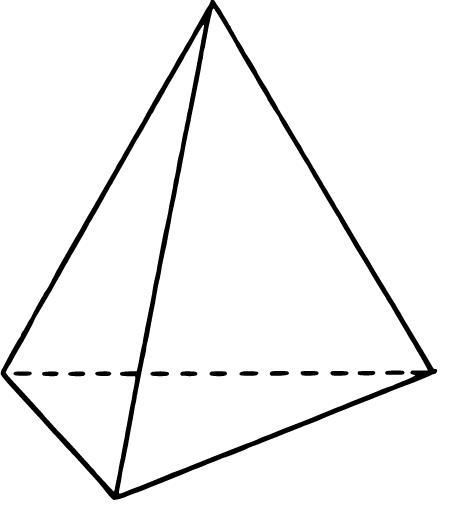
\includegraphics[width = 12cm]{Figuras/Taetraedro_Exemplo.jpg}
}
\subfigure[Molécula de DNA]{
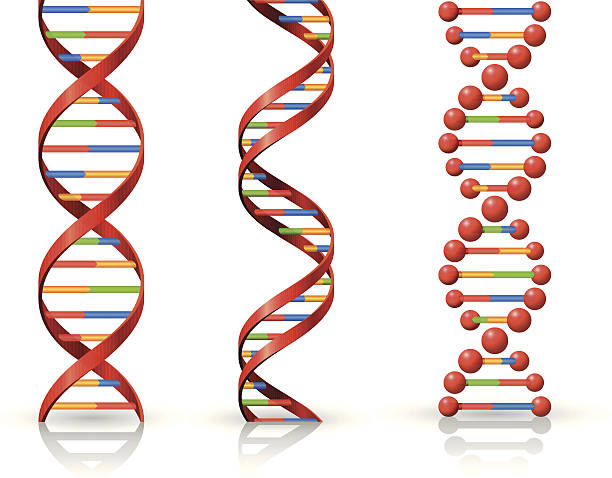
\includegraphics[width = 16.7cm]{Figuras/DNA_Exemplo.jpg}
}
\caption{ example of figures}
\end{center}
\end{figure}

Cras scelerisque suscipit pellentesque. Vivamus accumsan diam at interdum semper. Vivamus vestibulum imperdiet maximus. Cras mollis ultricies leo. Class aptent taciti sociosqu ad litora torquent per conubia nostra, per inceptos himenaeos. Nunc in lobortis enim.

\begin{table}[h!]
    \centering
    \begin{tabular}{|c|c|}
    \hline
         $n$ & Razão entre $a_{n+1}/a_{n}$  \\
    \hline
        $1$ & $1$\\ 
    \hline
         $2$ &  $2$\\
    \hline
        $3$ & $1.5$\\
    \hline
        $4$ & $1.666$\\
        \hline
        $5$ & $1.6$\\
        \hline
    \end{tabular}
    \caption{Razão entre os números da sequência de Fibonacci, onde $a_n$ representa o $n-$ésimo termo.}
\end{table}

Suspendisse imperdiet mollis velit nec tincidunt. Vivamus laoreet nulla non magna hendrerit, non dignissim enim porta. Quisque eget ex odio. Vestibulum non ex mollis, sodales nunc ut, varius quam. Aliquam fringilla convallis nulla.

 Suspendisse diam nisl, mattis nec volutpat sit amet, vestibulum vitae diam. Suspendisse ultrices ac est eu feugiat. Fusce ut efficitur purus. Curabitur suscipit nisi ut fermentum pretium. Suspendisse potenti.
